\section{Projective Representation of Configuration Algebra}\label{sec:projective-rep}
\begin{figure}
    \centering
    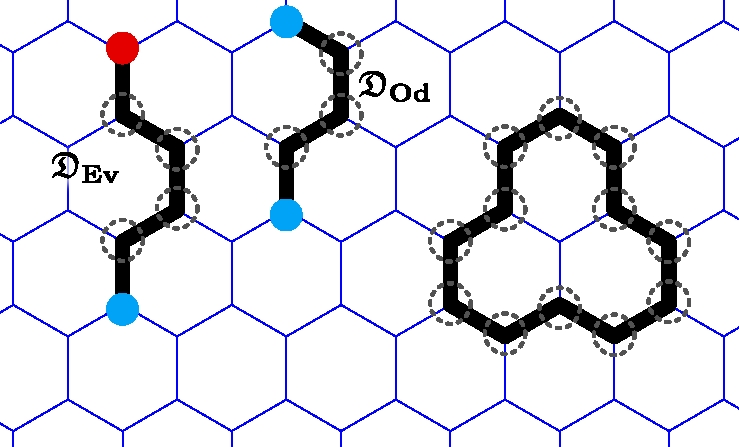
\includegraphics[width=0.8\linewidth]{figures/joints.pdf}
    \caption{The number of joints determines the factor $\eta_\mathfrak{D}$ of a edge configuration $\mathfrak{D}$. Each joint, marked by dashed circles in the figure, contributes a factor $\pm i$ due to the algebra of Pauli spin operators. The string $\mathfrak{D}_{\bo{Ev}}$ has two endpoints sitting in different sublattices, and there are an even number  (four, in this example) of joints on the string. In contrast, both endpoints of the string $\mathfrak{D}_{\bo{Od}}$ are in the same sublattice, and there are an odd number (three, in this example) of joints on the string. A loop, located at the right portion of the figure, doesn't have endpoints, and there are always an even number of joints on a closed loop.
    }
    \label{fig:joints}
\end{figure}

In this appendix, we rigorously discuss fundamental properties of the phase factor $\varphi(\mathfrak{D},\mathfrak{D}')$, defined in Eq.~\eqref{equ.Sigma-representation}, that emerges from the projective representation generated by string operators introduced in Sec.~\ref{sec:density-matrix-whole}.

\begin{definition}\label{def:Teven-odd}
  Given a class $[\mathfrak{D}]$, we denoted by $n_a(\mathfrak{D})$ and $n_b(\mathfrak{D})$  the number of $A$-sublattice sites and $B$-sublattice sites in $\mrm{Ed}\lr{\mathfrak{D}}$, respectively. The difference in number between sublattice $A$ and $B$ is indicated by $\Delta(\mathfrak{D}) \equiv n_a(\mathfrak{D})-n_b(\mathfrak{D})$. A class is said to be in the set $\TReven$ if and only if $n_a(\mathfrak{D})-n_b(\mathfrak{D}) \in 4\mathbb{Z}$. Otherwise, it is in the set $\TRodd$. That is,
  \[
  \TReven := \lrg{[\mathfrak{D}] \; :\; n_a(\mathfrak{D})-n_b(\mathfrak{D}) \in 4\mathbb{Z}} 
  \]
  We further define a phase factor $\eta_{\mathfrak{D}} \equiv (-1)^{\Delta(\mathfrak{D})/2}$ to distinguish $\TReven$ and $\TRodd$, that is
  \[
  \eta_\mathfrak{D}\equiv (-1)^{\Delta(\mathfrak{D})/2} = \begin{cases}
                       +1, & [\mathfrak{D}]\in\TReven \\
                       -1, & [\mathfrak{D}]\in\TRodd
                     \end{cases}
  \]
\end{definition}
\begin{definition}\label{def:good-def}
  Given a class $[\mathfrak{D}]\in\TReven$, such a class is said to be in a set $\Good$ if and only if $n_a(\mathfrak{D})=n_b(\mathfrak{D})$. That is,
  \[
  \Good = \lrg{[\mathfrak{D}] \; : \; n_a(\mathfrak{D}) = n_b(\mathfrak{D})}
  \]
  A configuration class in $\Good$ is said to be a \emph{good} configuration class. Note that the coefficients $\mathfrak{C}_{\mathfrak{D}}\neq 0$ iff $[\mathfrak{D}]\in\Good\subset\TReven$ due to Wick's theorem.
\end{definition}

% \begin{theorem}
%   Given $n$ good configuration classes $[\mathfrak{D}_1],\cdots,[\mathfrak{D}_n]\in\Good$ satisfy $[\mathfrak{D}_1\ominus\cdots\ominus\mathfrak{D}_n] = [\varnothing]$, the following relation holds,
%   \[
%   \prod_{i=1}^{n}\eta_{\mathfrak{D}\ominus\mathfrak{D}'} = (\eta_{\mathfrak{D}'})^n
%   \]
%   for an arbitrary configuration class $[\mathfrak{D}']$.
% \end{theorem}
% The proof of this theorem is straightforward.

In the following, we discuss the phase factor $\varphi(\mathfrak{D},\mathfrak{D}')$ of the projective representation of the configuration algebra and its relationship with the $\eta_\mathfrak{D}$ factors and the string operators $\Sigma_{\mathfrak{D}}$. First, we introduce a lemma that directly relates the string operators and the $\eta_{\mathfrak{D}}$ factors.
\begin{lemma}\label{lemma:sigma-eta-relation}
The factor $\eta_\mathfrak{D}$ is determined by the square of the corresponding string operator as follows.
  \[
  \Sigma_\mathfrak{D}^2 = \eta_{\mathfrak{D}} \mathds{1}
  \]
\end{lemma}
\begin{proof}
    Let $\mathsf{S}$ be an element of the projective Pauli group $\mathcal{P}_N \equiv \lrg{\mathds{1}, \sigma^x, \sigma^y, \sigma^z}^{\otimes N}$ of size $N$, which is the traditional Pauli group without phases $\lrg{\pm 1, \pm i}$. We define $\mathsf{S}_{\mathfrak{D}} \in \mathcal{P}_N$ as an operator that is proportional to the string operator corresponding to the same edge configuration $\mathsf{S}_\mathfrak{D} = \omega_\mathfrak{D} \Sigma_\mathfrak{D}$, where $\omega_\mathfrak{D}\in\lrg{\pm1, \pm i}$ is a phase factor arising from the algebra of Pauli spin operators. According to the definition of the string operator given by Eq.~\eqref{equ.string-operator-def}
    and the structure of strings illustrated in \autoref{fig:joints}, one can see that each joint on the string contributes a $\pm i$ to the phase factor $\omega_\mathfrak{D}$ due to the algebra $\sigma^\mu\sigma^\nu = i\epsilon^{\mu\nu\lambda}\sigma^\lambda$. Combining this conclusion and the fact that every element in $\mathcal{P}_N$ squares to one, we obtain the following relation for $\eta_\mathfrak{D}$,
    \[
    \eta_\mathfrak{D} = \omega_\mathfrak{D}^2 = \lrm{(\pm i)^{2}}^{\text{\# of joints}} = (-1)^{\text{\# of joints}}.
    \]
    edge configurations $\mathfrak{D}$ consisting of a single simply-connected string with two endpoints can be divided into two types. The first type, which is a subset of $\TReven$, consists of strings with both endpoints in the same sublattice, while the second type, which is a subset of $\TRodd$, consists of strings with two endpoints in different sublattices. According to \autoref{fig:joints}, the strings in $\TReven$ have an even number of joints; hence, the corresponding phase factor is $\eta_\mathfrak{D} = 1$. In contrast, the strings in $\TRodd$ have an odd number of joints; hence, the corresponding phase factor is $\eta_\mathfrak{D} = -1$. Consider a $\TReven$-edge configuration with $n_a(\mathfrak{D}) - n_b(\mathfrak{D}) \in 4\mathbb{Z}$, the four integers of the endpoints of the same sublattice type come from the two integers of strings possessing two endpoints in the same sublattice. Therefore, the negative factor $\eta$ from these two integers of strings cancel each other, leaving the overall phase $\eta_\mathfrak{D} = +1$. In contrast, if $\mathfrak{D} \in \TRodd$, the negative phases cannot be canceled and the overall phase will be left with a negative sign $\eta_\mathfrak{D} = -1$. This completes the proof.
\end{proof}
\begin{corollary}
    A string operator $\Sigma_\mathfrak{D}$ squares to one if $\mathfrak{C}_\mathfrak{D} \neq 0$ in the pure Kitaev model.
\end{corollary}
\begin{proof}
    As mentioned in Definition~\ref{def:good-def}, a necessary and sufficient condition for a edge configuration $\mathfrak{D}$ to have a finite correlation function $\mathfrak{C}_\mathfrak{D} \neq 0$ is $[\mathfrak{D}] \in \Good$. Because $\Good\subset\TReven$, the phase factor of $[\mathfrak{D}] \in \Good$ must be positive by definition, $\eta_\mathfrak{D} = +1$. Owing to this, according to Lemma~\ref{lemma:sigma-eta-relation},  
    \[
    \Sigma_\mathfrak{D}^2 = \eta_\mathfrak{D}\mathds{1} = \mathds{1}
    \]
    if $[\mathfrak{D}]\in\Good$. This completes the proof.
\end{proof}

These string operators form a projective representation of the algebra $\anglelr{\lrg{\mathfrak{D}}, \ominus}$ for edge configurations as follows,
\begin{equation}\label{eq:phi-phase-factor-def}
  \Sigma_{\mathfrak{D}}\Sigma_{\mathfrak{D}'} = \varphi(\mathfrak{D},\mathfrak{D}') \Sigma_{\mathfrak{D}\ominus\mathfrak{D}'},
\end{equation}
where $\varphi(\mathfrak{D},\mathfrak{D}')\in\lrg{-1,1}$ is the phase factor of the projective representation. 
%The fact that the multiplications among string operators preserve the structure of the algebra $\anglelr{\lrg{\mathfrak{D}},\ominus}$ can be verified straightforwardly given the property $[\mathcal{P}^{(p)}, \Sigma_{\mathfrak{D}}] = 0$ and Eq.~\eqref{eq:phi-phase-factor-def}. Because $\mathcal{S}_\mathfrak{D}$ depends only on the equivalence class $[\mathfrak{D}]$, the elements in the algebra are therefore the equivalence classes.
\begin{theorem}\label{cor:phase-associativity}
  Due to the associativity of the representation, the following relation holds for three arbitrary edge configurations $\mathfrak{D}$, $\mathfrak{D}'$, and $\mathfrak{D}''$,
\[
\varphi(\mathfrak{D},\mathfrak{D}'\ominus\mathfrak{D}'')\varphi(\mathfrak{D}',\mathfrak{D}'') = 
\varphi(\mathfrak{D},\mathfrak{D}')\varphi(\mathfrak{D}\ominus\mathfrak{D}',\mathfrak{D}'').
\]
\end{theorem}

\begin{theorem}\label{thm:phi-operational-def}
The phase factor defined in Eq.~\eqref{eq:phi-phase-factor-def} can be reformulated as follows,
\[
\varphi(\mathfrak{D},\mathfrak{D}') = \frac{1}{2^{N}}\eta_{\mathfrak{D}\ominus\mathfrak{D}'}\Tr\lrm{\Sigma_{\mathfrak{D}}\Sigma_{\mathfrak{D}'}\Sigma_{\mathfrak{D}\ominus\mathfrak{D}'}}.
\]
\end{theorem}
\begin{proof}
First, convert the multiplication of the first two string operators $\Sigma_\mathfrak{D}$ and $\Sigma_{\mathfrak{D}'}$ into the string operator $\Sigma_{\mathfrak{D}\ominus\mathfrak{D}'}$ of the resulting configuration using the definition of the phase factor Eq.~\eqref{eq:phi-phase-factor-def}
\[
\Tr\lrm{\Sigma_{\mathfrak{D}}\Sigma_{\mathfrak{D}'}\Sigma_{\mathfrak{D}\ominus\mathfrak{D}'}}
= \varphi(\mathfrak{D},\mathfrak{D}')\Tr\lrm{\Sigma_{\mathfrak{D}\ominus\mathfrak{D}'}\Sigma_{\mathfrak{D}\ominus\mathfrak{D}'}}
\]
According to Lemma~\ref{lemma:sigma-eta-relation}, the square of the string operator in the trace reduces to the $\eta$ factor
\[
\Tr\lrm{\Sigma_{\mathfrak{D}\ominus\mathfrak{D}'}\Sigma_{\mathfrak{D}\ominus\mathfrak{D}'}}
=
\varphi(\mathfrak{D},\mathfrak{D}')\Tr\lr{\mathds{1}}\eta_{\mathfrak{D}\ominus\mathfrak{D}'}.
\]
Combining the two equations completes the proof.
\end{proof}

\begin{lemma}\label{g-self.thm}
 Given an arbitrary edge configuration $\mathfrak{D}$, the following two relations hold.
 
\begin{enumerate}
    \item [(i)] $\varphi(\varnothing, \mathfrak{D}) = \varphi(\mathfrak{D},\varnothing)= 1$
    \item [(ii)] $\varphi(\mathfrak{D},\mathfrak{D}) = \eta_{\mathfrak{D}}$
\end{enumerate}
\begin{proof}
    The first relation comes from Eq.~\eqref{eq:phi-phase-factor-def} and the fact that $\Sigma_\varnothing = \mathds{1}$. The second relation is equivalent to Lemma~\ref{lemma:sigma-eta-relation} reformulated using the factor $\phi$ given in Eq.~\eqref{eq:phi-phase-factor-def}.
\end{proof}
\end{lemma}

\begin{lemma}\label{g-reduce-theorem.thm}
Given two arbitrary edge configurations $\mathfrak{D}$ and $\mathfrak{D}'$, the following two equations hold.
\begin{enumerate}
    \item [(i)] $\varphi(\mathfrak{D},\mathfrak{D}\ominus\mathfrak{D}') = \eta_{\mathfrak{D}'}\eta_{\mathfrak{D}\ominus\mathfrak{D}'} \varphi(\mathfrak{D}',\mathfrak{D})$
    \item [(ii)] $\varphi(\mathfrak{D}\ominus\mathfrak{D}',\mathfrak{D}) = \eta_{\mathfrak{D}'}\eta_{\mathfrak{D}\ominus\mathfrak{D}'} \varphi(\mathfrak{D},\mathfrak{D}')$.
\end{enumerate}
\end{lemma}
\begin{proof}
Applying Theorem~\ref{thm:phi-operational-def} directly, we have
  \begin{align*}
    \varphi(\mathfrak{D},\mathfrak{D}\ominus\mathfrak{D}') &= \frac{\eta_{\mathfrak{D}\ominus\mathfrak{D}\ominus\mathfrak{D}'}}{2^{N}}\Tr\lrm{\Sigma_{\mathfrak{D}}\Sigma_{\mathfrak{D}\ominus\mathfrak{D}'}\Sigma_{\mathfrak{D}\ominus\mathfrak{D}\ominus\mathfrak{D}'}} \\
    &= \frac{\eta_{\mathfrak{D}'}}{2^{N}}\Tr\lrm{\Sigma_{\mathfrak{D}}\Sigma_{\mathfrak{D}\ominus\mathfrak{D}'}\Sigma_{\mathfrak{D}'}} \\
    &= \frac{\eta_{\mathfrak{D}'}}{2^{N}}\Tr\lrm{\Sigma_{\mathfrak{D}'}\Sigma_{\mathfrak{D}}\Sigma_{\mathfrak{D}'\ominus\mathfrak{D}}} \\
    &=\eta_{\mathfrak{D}'}\eta_{\mathfrak{D}'\ominus\mathfrak{D}} \varphi(\mathfrak{D}',\mathfrak{D}).
  \end{align*}
The result proves the first equation of the lemma. A similar approach leads to the second equation of the lemma.
\end{proof}
\begin{lemma}\label{g_reduce_symmetric.e}
Given two arbitrary edge configurations $\mathfrak{D}$ and $\mathfrak{D}'$, the following relation holds,
  \[
  \varphi(\mathfrak{D}, \mathfrak{D}\ominus\mathfrak{D}') = \eta_{\mathfrak{D}}\varphi(\mathfrak{D},\mathfrak{D}').
  \]
\end{lemma}
\begin{proof}
  According to Theorem~\ref{cor:phase-associativity}, the associativity of the projective representation implies
  \[
  \varphi(\mathfrak{D},\mathfrak{D}\ominus\mathfrak{D}')\varphi(\mathfrak{D},\mathfrak{D}') = \varphi(\mathfrak{D},\mathfrak{D})\varphi(\mathfrak{D}\ominus\mathfrak{D},\mathfrak{D}')
  \]
  According to Lemma \ref{g-self.thm}, the terms on the right-hand side of the equation can be replaced by $\eta$ factors. Therefore, the above relation reduces to the following,
  \[
  \varphi(\mathfrak{D},\mathfrak{D}\ominus\mathfrak{D}')\varphi(\mathfrak{D},\mathfrak{D}') = \eta_{\mathfrak{D}}.
  \]
  Since $\varphi,\eta = \pm 1$, we obtain
  \[
  \varphi(\mathfrak{D},\mathfrak{D}\ominus\mathfrak{D}') = \eta_{\mathfrak{D}}\varphi(\mathfrak{D},\mathfrak{D}').
  \]
  This completes the proof.
\end{proof}
\begin{theorem}\label{theorem:phi_exchange}
Given two arbitrary edge configurations $\mathfrak{D}$ and $\mathfrak{D}'$, the sign factor produced by exchanging the positions of the two configurations in $\varphi(\mathfrak{D},\mathfrak{D}')$ is determined by $\eta$ factors as follows,
  \[
  \varphi(\mathfrak{D},\mathfrak{D}') = \eta_{\mathfrak{D}}\eta_{\mathfrak{D}'}\eta_{\mathfrak{D}\ominus\mathfrak{D}'} \varphi(\mathfrak{D}',\mathfrak{D}) .
  \]
\end{theorem}
\begin{proof}
  Combining Lemmas \ref{g-reduce-theorem.thm} and \ref{g_reduce_symmetric.e} leads to the following equation,
  \[
  \varphi(\mathfrak{D},\mathfrak{D}\ominus\mathfrak{D}') = 
  \eta_{\mathfrak{D}'}\eta_{\mathfrak{D}\ominus\mathfrak{D}'} \varphi(\mathfrak{D}',\mathfrak{D}) =
  \eta_{\mathfrak{D}}\varphi(\mathfrak{D},\mathfrak{D}').
  \]
  Such an equation leads to the equation of this theorem.
\end{proof}
\begin{corollary}
The phase factor due to the exchange of two string operators can be determined by the corresponding factors $\eta$ as follows.
  \[
  \Sigma_{\mathfrak{D}}\Sigma_{\mathfrak{D}'} = \eta_{\mathfrak{D}}\eta_{\mathfrak{D}'}\eta_{\mathfrak{D}\ominus\mathfrak{D}'} 
  \Sigma_{\mathfrak{D}'}\Sigma_{\mathfrak{D}}.
  \]
\end{corollary}

% \begin{corollary}
%   \[
%   \eta_{\mathfrak{D}\ominus\mathfrak{D}'} = \varphi(\mathfrak{D}\ominus\mathfrak{D}',\mathfrak{D}) \varphi(\mathfrak{D}\ominus\mathfrak{D}',\mathfrak{D}')
%   \]
% \end{corollary}
% \begin{proof}
%   From 
%   $
%   \eta_{\mathfrak{D}\ominus\mathfrak{D}'} = \eta_{\mathfrak{D}}\eta_{\mathfrak{D}'} \varphi(\mathfrak{D}',\mathfrak{D}) \varphi(\mathfrak{D},\mathfrak{D}')
%   $, 
%   substitute $\varphi(\mathfrak{D},\mathfrak{D}') = \eta_{\mathfrak{D}} \eta_{\mathfrak{D}\ominus\mathfrak{D}'}\varphi(\mathfrak{D}\ominus\mathfrak{D}',\mathfrak{D})$, we then prove this corollary.
% \end{proof} 